\documentclass{article}


\usepackage{graphicx}
\usepackage{listings}
\usepackage{amsmath}
\usepackage{wrapfig}
\usepackage[bookmarks]{hyperref}
\usepackage[table,xcdraw]{xcolor}
\usepackage{geometry}
\usepackage{pdfpages}
\usepackage{fancyhdr}
\usepackage{xepersian}

\settextfont{XW Zar}

\geometry{
  right = 30 mm,
  left = 25mm,
  top = 35mm,
  bottom = 30mm,
}

\pagestyle{fancy}
\rhead{\textbf{محمد حسین امینی}}
\lhead{\rightmark}

\linespread{1.1}
\hypersetup{
	colorlinks=true,
	linkcolor=black,
	filecolor=magenta,      
	urlcolor=cyan,
}

\lstset{
	language=Python,
	basicstyle=\setLTR\ttfamily\large,
	aboveskip={1.0\baselineskip},
	belowskip={1.0\baselineskip},
	columns=fixed,
	extendedchars=true,
	breaklines=true,
	tabsize=4,
	prebreak=\raisebox{0ex}[0ex][0ex]{\ensuremath{\hookleftarrow}},
	frame=lines,
	showtabs=false,
	showspaces=false,
	showstringspaces=false,
	keywordstyle=\color[rgb]{0.627,0.126,0.941},
	commentstyle=\color[rgb]{0.133,0.545,0.133},
	stringstyle=\color[rgb]{01,0,0},
	numbers=left,
	numberstyle=\small,
	stepnumber=1,
	numbersep=10pt,
	captionpos=t,
	escapeinside={\%*}{*)}
}



\begin{document}

	\begin{titlepage} 
		\centering  
		
\includegraphics [width = 0.15 \textwidth] {AUT.png} \par \vspace { 0cm }
				{ \scshape \LARGE 
					دانشگاه صنعتی امیرکبیر (پلی تکنیک تهران)\\
					دانشکده مهندسی برق
					\par }
		\vspace { 2cm } 
		{ \Huge \bfseries 
پروژه کارشناسی
			\par } 
		\vspace { 4cm } 
		{ \huge
			محمد حسین امینی  -  محمد مهدی مرادی
			 } 
		\vfill 
		{ \huge
استاد راهنما:
\par 
دکتر محمد اعظم خسروی - دکتر ابوالقاسم اسداله راعی
		}
		\vfill
		 
		% Bottom of the page 
		\vspace { 2cm } 
		%{ \large  سال 1397 \par } 
	\end{titlepage} 
\newpage
\begin{figure}[h!]

\includegraphics[width=\textwidth]{A3.png}
\end{figure}
\begin{flushleft}
{
\LARGE
وَفَوْقَ كُلِّ ذِي عِلْمٍ عَلِيمٌ...\\
}
{
\large
سوره مبارکه یوسف (ع) - آیه 76
}
\end{flushleft}


\newpage
{\Large\tableofcontents}
\newpage
{\Large\section{مقدمه}
\newpage
\section{پردازش تصویر ورودی}
تصاویر در کامپیوتر به دو صورت ذخیره می شوند:\\
\begin{enumerate}
\item \lr{Raster Graphics}\\
توضیحات...
\item \lr{Vector Graphics}\\
توضیحات...
\end{enumerate}
در دستگاه هایی همچون 
\lr{Printer} 
ها به دلیل نحوه عملکرد دستگاه، تصاویر باید در قالب 
\lr{Raster}
وارد دستگاه شوند؛ اما در دستگاه هایی چون روبات های نقاش با توجه به طبیعت این روبات ها، به تصاویر 
\lr{Vectorized}
نیازمندیم. از طرفی با توجه به این که  خروجی اکثر وسایل تصویربرداری از جمله دوربین های دیجیتال و همچنین تصاویر ذخیره شده در کامپیوتر بصورت 
\lr{Raster}
هستند در اولین گام به تبدیل تصاویر 
\lr{Raster}
به 
\lr{Vectorized}
پرداخته ایم.
\subsection{\lr{OpenCV}}
جهت پیاده سازی الگوریتم های پردازش تصویر از ماژول 
\lr{OpenCV}
در پایتون استفاده شده است. ابتدا به معرفی کلی این ماژول می پردازیم و سپس توابع استفاده شده از آن را توضیح می دهیم.
\subsubsection{معرفی کلی 
\lr{OpenCV}
}
توضیحات...
\subsubsection{تابع
\lr{imread}
}
توضیحات...
\subsubsection{تابع
\lr{fastNlMeansDenoisingColored}
}
توضیحات...
\subsubsection{تابع
\lr{cvtColor}
}
توضیحات...
\subsubsection{تابع
\lr{adaptiveThreshold}
}
توضیحات...
\subsubsection{تابع
\lr{findContours}
}
توضیحات...

\subsubsection{تابع
\lr{drawContours}
}
توضیحات...


\subsection{پیش پردازش}
جهت توضیحات بهتر مراحل لازم در مرحله پیش پردازش را با شکل
\ref{fig:Sample6}
انجام می دهیم و خروجی هر مرحله را نمایش می دهیم.\\
\begin{figure}[h!]
 \centering 
 
\includegraphics[width=0.5\textwidth]{Sample6.jpg}
 \caption{تصویر ورودی جهت پیش پردازش}
 \label{fig:Sample6}
\end{figure}
ابتدا لازم است تا لبه
\LTRfootnote{Edge}
 ها و کانتور
\LTRfootnote{Contour}
 های تصویر را بدست آوریم. جهت افزایش کیفیت کار، ابتدا به کاهش نویز موجود در تصویر می پردازیم که خروجی آن را در شکل
\ref{fig:Denoised}
می بینیم.
\begin{figure}[h!]
 \centering 
 
\includegraphics[width=0.5\textwidth]{DenoisedSample6.jpg}
 \caption{خروجی حاصل از کاهش نویز تصویر}
 \label{fig:Denoised}
\end{figure}
  پس از مرحله کاهش نویز، جهت یافتن کانتور ها ابتدا تصویر را به فرمت سیاه و سفید
\LTRfootnote{Grayscale}
تبدیل می کنیم که خروجی حاصل را در شکل 
\ref*{fig:Grayscaled}
می بینیم.\\
\begin{figure}[h!]
  \centering 
  
\includegraphics[width=0.5\textwidth]{GrayscaleSample6.jpg}
  \caption{خروجی حاصل از سیاه و سفید کردن تصویر}
  \label{fig:Grayscaled}
 \end{figure}
سپس عملیات 
\lr{Thresholding}
را بر روی آن اعمال می کنیم. خروجی حاصل از این عملیات درشکل
\ref{fig:Thresholded}
آمده است.
 \begin{figure}[h!]
  \centering 
  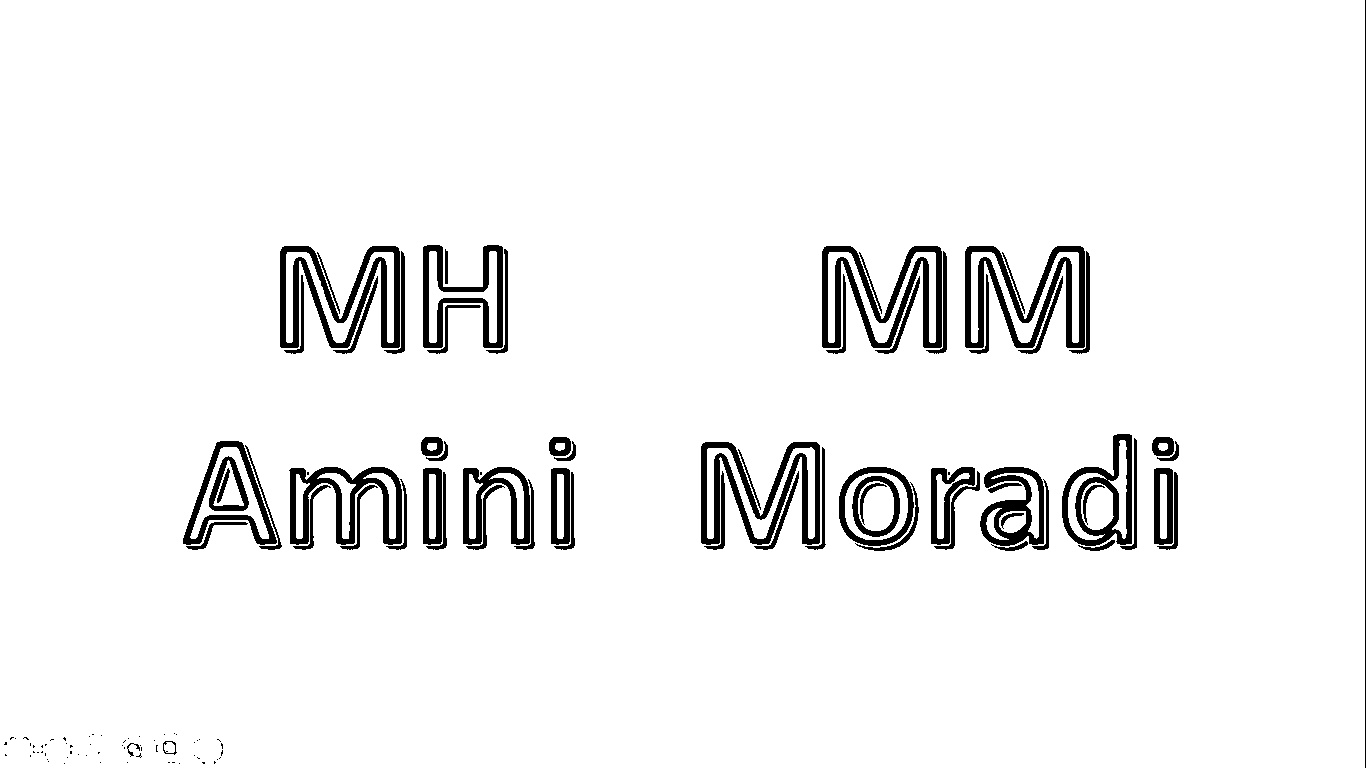
\includegraphics[width=0.5\textwidth]{ThresholdedSample6.jpg}
  \caption{خروجی حاصل از عملیات 
  \lr{Thresholding}
  }
  \label{fig:Thresholded}
 \end{figure}
پس از عملیات
\lr{Thresholding}
نوبت به یافتن کانتور های تصویر می رسد. با انجام این عملیات نقاط متوالی مربوط به هر کانتور را در قالب یک 
\lr{List}
پایتون خواهیم داشت که جهت هدایت روبات از این نقاط استفاده خواهیم کرد.

 \begin{figure}[h!]
  \centering 
  
\includegraphics[width=0.5\textwidth]{ContoursSample6.jpg}
  \caption{خروجی حاصل از یافتن کانتور ها }
  \label{fig:Contours}
 \end{figure}
\pagebreak
\subsubsection{کد های پیش پردازش تصویر}
\begin{lstlisting}
##  Image file name...
filename='Sample6.jpg'

##  Reading the image...
im = cv2.imread(filename)
page_size=[im.shape[0], im.shape[1]]
page_center=[int(page_size[0]/2),int(page_size[1]/2)]

##  Denoising the image...
dst = cv2.fastNlMeansDenoisingColored(im,None,10,10,7,21)
cv2.imwrite('Denoised{}'.format(filename),dst)

##  Grayscaling the image...
imgray = cv2.cvtColor(dst,cv2.COLOR_BGR2GRAY)
cv2.imwrite('Grayscale{}'.format(filename),imgray)

##  Thresholding the image...
thresh = cv2.adaptiveThreshold(imgray,255,cv2.ADAPTIVE_THRESH_GAUSSIAN_C,
                               cv2.THRESH_BINARY,15,2)
cv2.imwrite('Thresholded{}'.format(filename),thresh)

##  Finding the image contours...
im2, contours, hierarchy = cv2.findContours(thresh,cv2.RETR_TREE,cv2.CHAIN_APPROX_SIMPLE)

##  Sorting contours...
contours = sorted(contours, key=cv2.contourArea, reverse = True)[:10]

imcontours=im.copy()
cv2.drawContours(imcontours, contours, -1, (0,255,0), 3)
cv2.imwrite('Contours{}'.format(filename),imcontours)

\end{lstlisting}

}
\end{document}
